\section{Démarche Expérimentale}

\begin{wrapfigure}{R}{0.6\linewidth}
    \centering
    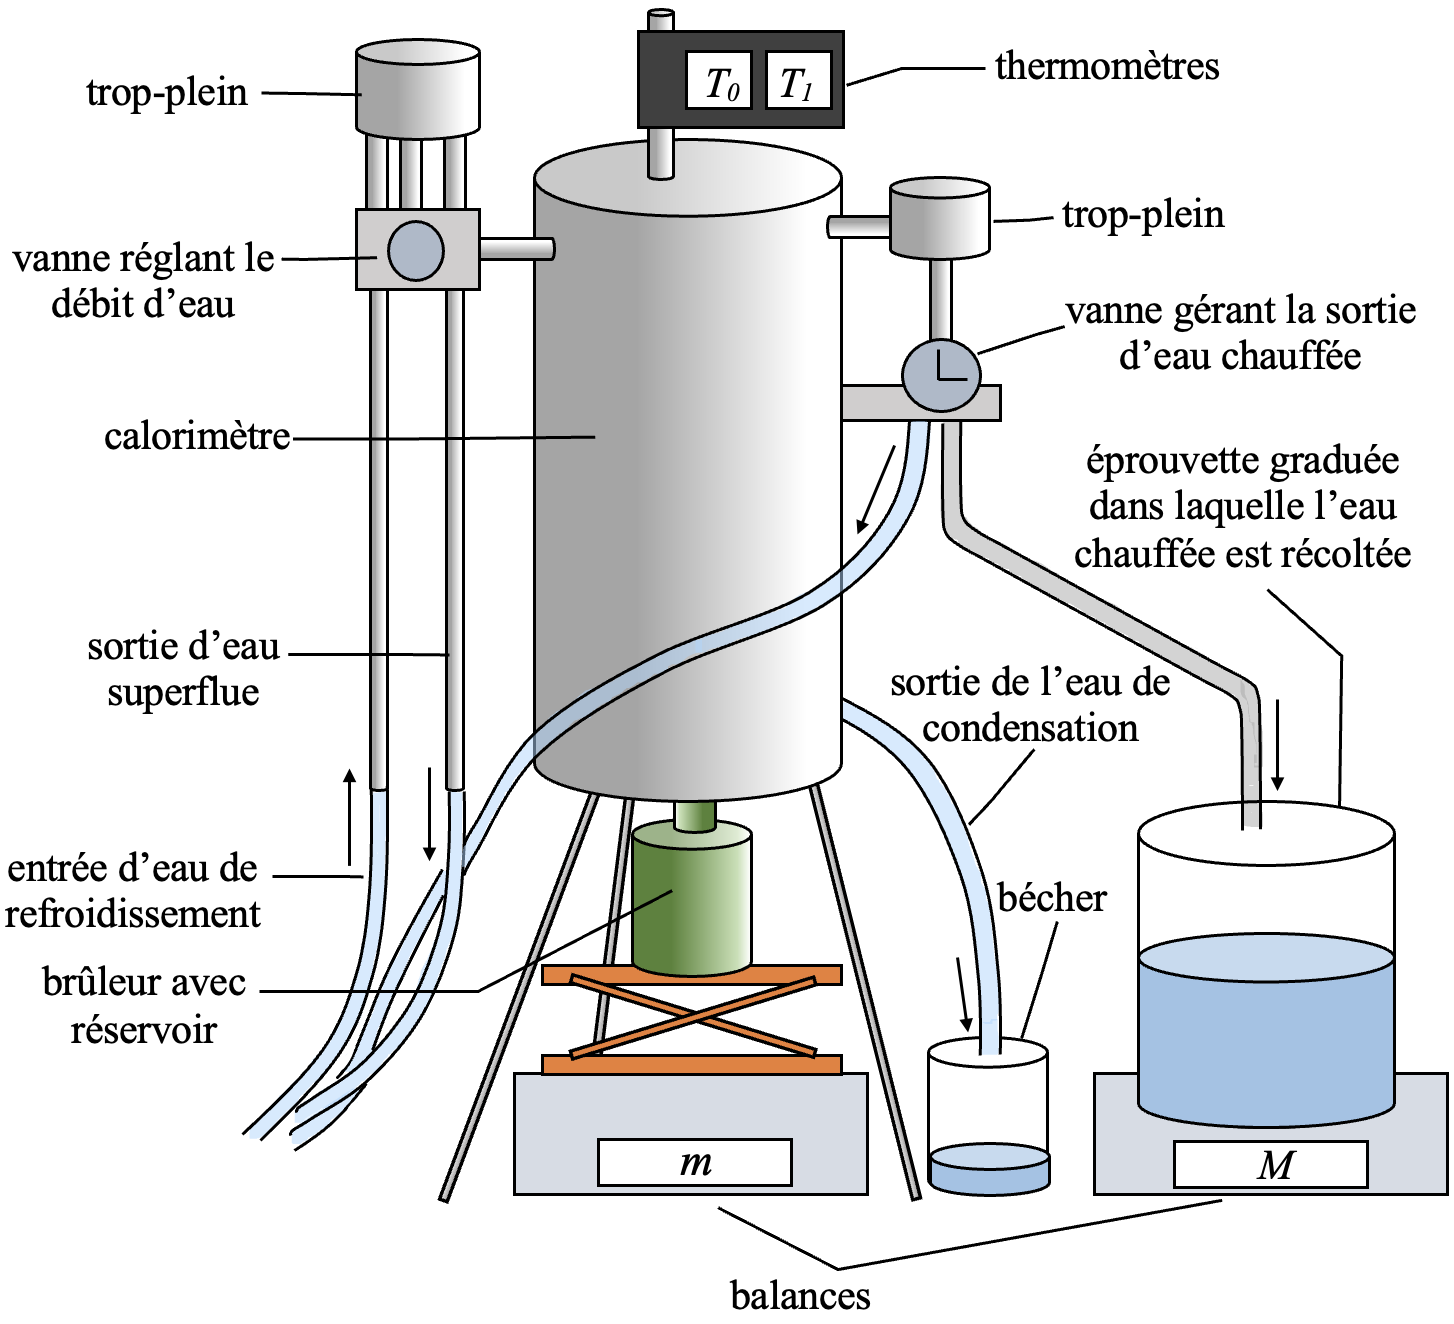
\includegraphics[width=\linewidth]{figures/montage.png}
    \caption{Montage expérimental \cite{rapport-mendels-pascaud}}
    \label{fig:montage}
\end{wrapfigure}

\paragraph*{Calorimetrie}
Afin de déterminer le pouvoir calorifique des combustibles le montage à la \autoref{fig:montage} est utilisé. Le calorimetre échangeur de chaleur est un appareil permettant de mesurer les échanges de chaleur entre deux fluides, sans pertes. Lors de cette expérience, la combustion entraine une augmentation de l'énergie interne du calorimetre \(\Delta U_1\), qui entraine une augmentation de l'énergie interne de l'eau \(\Delta U_2\). En considérant la combustion comme complète, puisqu'il y a un apport de \ce{O2} suffisant, la chaleur produite par la combustion est donnée par la somme de ces deux énergie internes, puisqu'aucun travail n'est effectué.
\begin{equation}
    \mathcal{Q} = \Delta U_1 + \Delta U_2
\end{equation}
Un état d'équilibre est atteint lorsque la différence entre la température d'entrée \(T_1\) et la température de sortie \(T_2\) reste constante. On a alors plus d'augmentation de l'énergie interne du calorimetre, c'est à dire que \(\Delta U_1 = 0\).

\paragraph*{Pouvoir calorifique}
Afin de mesurer le pouvoir calorifique des combustibles, un bruleur contenant le combustible à étudier est démaré, chauffant le calorimetre. Les mesures s'effectuent lorsque l'état d'équilibre est atteint. La masse d'eau \(\Delta M\) évacuée pour une certaine masse de combustible \(\Delta m\) sont mesurées à l'aide de balances digitales. L'écart de température entre l'entrée d'eau et la sortie sont relevés par des thermomètres. De plus, un bécher permet de récupérer l'eau de condensation produite au long de l'expérience. La masse d'eau condensée \(\Delta M_c\) est mesurée à la fin des mesures et divisée également sur toutes les mesures en raison de sa faible quantité. Le pouvoir calorifique du combustible est alors donné par la différence entre l'énergie \(\Delta U_2\) et l'énergie de la condensation de l'eau, pour une masse de combustible brulé.
\begin{equation}
    H = \frac{\Delta U_2 - \Delta M_c \ell_\textrm{vap}^*}{\Delta m} = \frac{c^* \Delta M (T_2 - T_1) - \Delta M_c \ell_\textrm{vap}^*}{\Delta m}
    \label{eq:pouvoir_calorifique}
\end{equation}
avec \(c^* = (4179.6 \pm 0.1)\) \si{\joule\per\kelvin\per\kilo\gram} la capacité thermique massique de l'eau \cite{capacite-eau} et \mbox{\(\ell_\textrm{vap}^* = 2257\) \si{\kilo\joule\per\kilo\gram}} la chaleur latente massique de vaporisation de l'eau \cite{notice}.

\paragraph*{Ecart théorique-expérimental}
Afin de comparer les valeurs théoriques et expérimentales, l'écart relatif est \(a\) utilisé. 
